\chapter{Techniczny opis programu} 
Narzędzie składa się z trzech głównych części:
\begin{itemize}
\item interfejsu użytkownika napisanego przy użyciu frameworku CSS'owego ,,Bootstrap'',
\item serwera napisanego w Node.js. Serwer jest uruchamiany lokalnie na urządzeniu użytkownika, komunikuje się z aplikacją internetową oraz interfejsem użytkownika,
\item aplikacji internetowej, napisanej we frameworku Google Apps Script po stronie Google'a, pod prywatnym kontem e-mailowym.


\end{itemize}
Poza tym lokalny serwer wykorzystuje kilka bibliotek JavaScriptowych oraz Pythonowych do dodatkowych obliczeń. Schemat połączeń w projekcie:
\begin{figure}[H]
  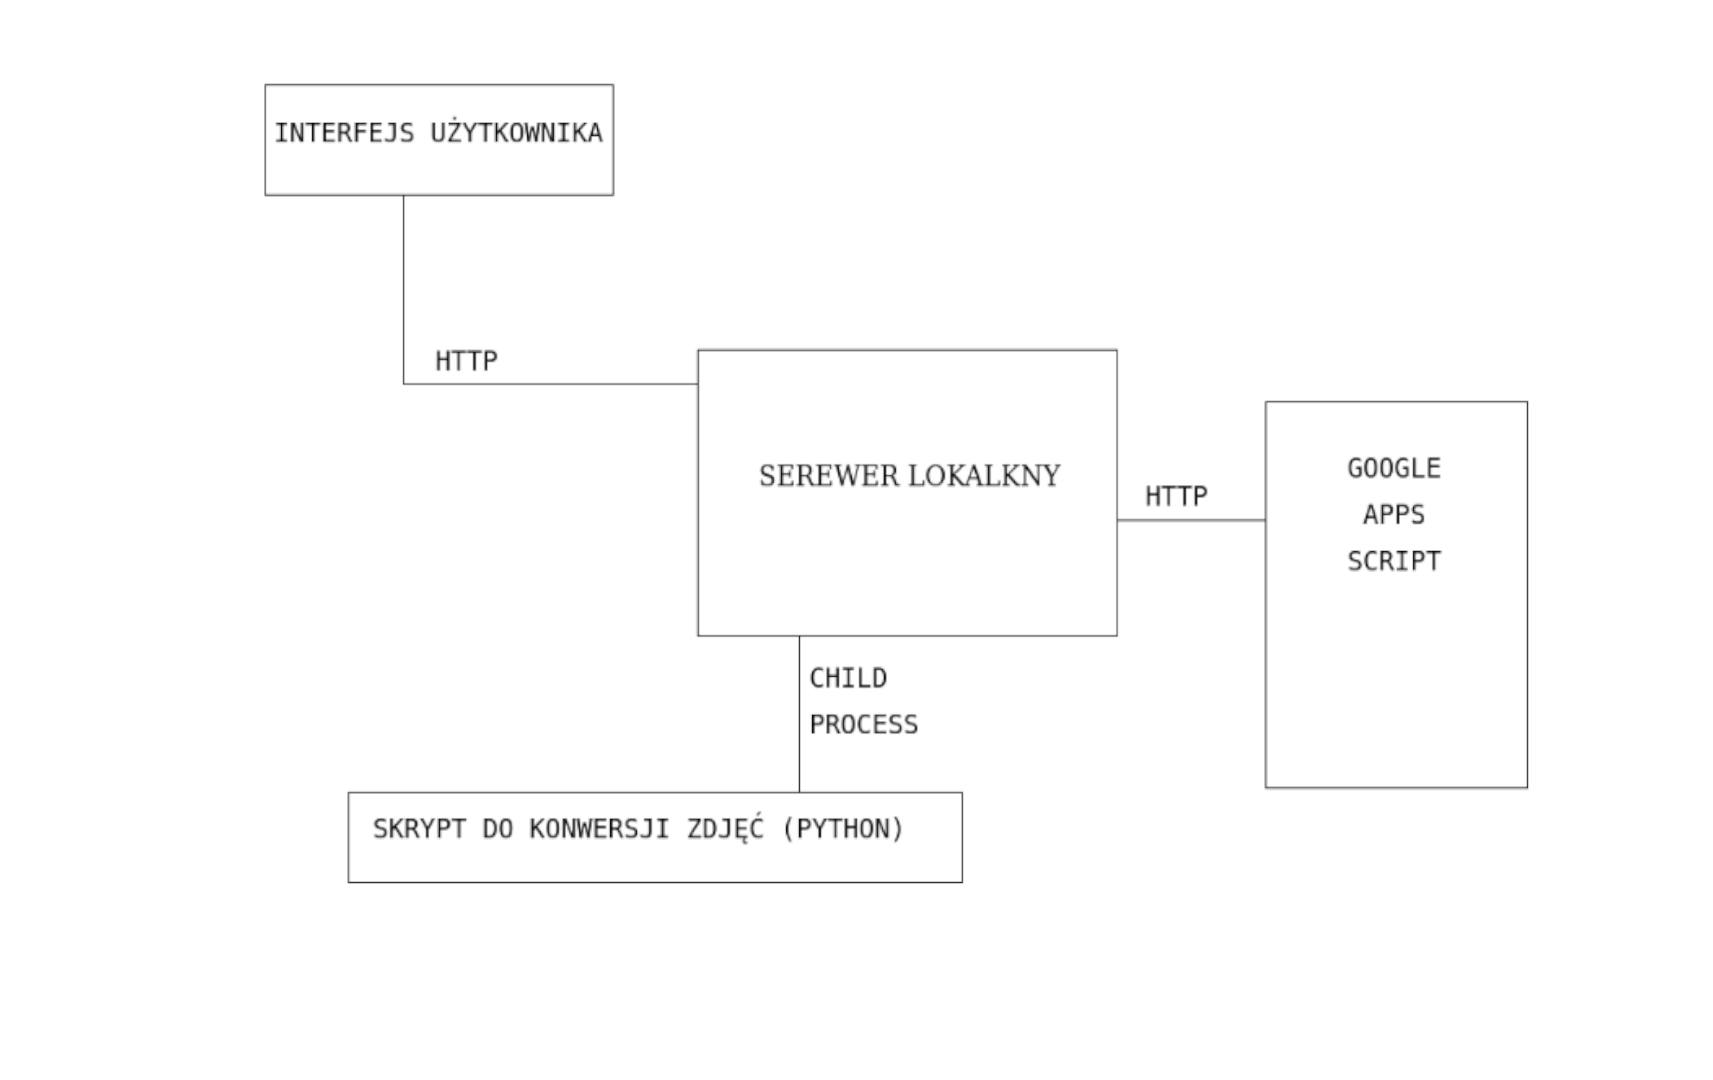
\includegraphics[scale=0.75]{schemat.png}
  \caption{Schemat połączeń}
  \label{fig:1}
\end{figure}
\section{Interfejs użytkownika}
Na interfejs użytkownika składają się trzy pliki: \textit{strona.html}, \textit{memoryFile.js} oraz \textit{htmlCode.js} -- pierwszy z nich koduje część wizualną, drugi dane na temat formularzy, trzeci jest odpowiedzialny za zachowanie poszczególnych elementów, w tym za komunikację z serwerem. 
\ind Elementami interfejsu są:
\begin{itemize}
\item pole do wgrywania plików, przyjmujące formaty .json oraz .txt. Zawartość powinna spełniać wymagania opisane w instrukcji w podrozdziale 4.2, %TODO link zrobić.
\item przycisk wgrywający plik -- ,,generate form'' wywołuje metodę getFile,
\item listę formularzy, w której poprzez kliknięcie można wybrać formularz,
\item kilka przycisków powiązanych z metodą getInfo().
\end{itemize}
\ind Plik \textit{memoryFile.js} jest modyfikowany przez serwer lokalny i służy do zapamiętywania formularzy utworzonych przez aplikację. Jako kod zawiera on wyłącznie deklarację stałej ,,memory'', będącej obiektem JSON następującej budowy:
\begin{figure}[H]
\begin{lstlisting}[language=json,firstnumber=1]
{"forms":
    [{"id": "string",
      "date": "string",
      "name": "string"}
    ]
}
\end{lstlisting}
\end{figure}
Wartość ,,id'' jest generowana przez usługę Google'a przy tworzeniu formularza, ,,date'' to data utworzenia formularza (rok-miesiąc-dzień), ,,name'' odpowiada tytułowi.
\ind Wartość ,,selectedForm'' z pliku \textit{htmlCode.js} odpowiada identyfikatorowi formularza obecnie podświetlonego na niebiesko na liście formularzy. Metody zaimplementowane w \textit{htmlCode.js}:
\begin{itemize}
\item changeLocation(newLocation) -- pozwala na zmianę wyświetlanego adresu,
\item makeHttpRequest(Url, callback) -- wysyła żądanie GET do lokalnego serwera (adres URL zależny jest od rodzaju przeprowadzanej akcji), w przypadku pozytywnej odpowiedzi (HTTP status 200) wywołuje metodę callback,
\item getInfo(action) -- metoda przypisana większości przycisków interfejsu, jest odpowiedzialna za odpowiednie wywołanie makeHttpRequest,
\item getFile() -- funkcja przypisana do przycisku ,,Generate form'', wczytuje wgrany plik, sprawdza, czy jest on poprawnym JSONem i wywołuje makeHttpRequest z odpowiednimi argumentami.
\item assign(id) -- metoda przypisana do elementów listy formularzy, ustawia wartość ,,selectedForm'' przy każdej zmianie wybranego z listy formularza,
\item generateList() -- tworzy listę formularzy na podstawie \textit{memoryFile.js}, jest uruchamiana przy ładowaniu strony.
\end{itemize}


\section{Serwer Node.js'owy}
Serwer to prosta implementacja aplikacji we frameworku ,,express.js''. Po uruchomieniu nasłuchuje na porcie 3000 (co można zmienić w pliku \textit{server.js}, linia 3). Możliwe są trzy odwołania do serwera:
\begin{itemize}
\item uploadJsonFile
\item createForm
\item getInfo
\end{itemize}
Aplikacja korzysta z bibliotek ,,express'', ,,cors'', ,,fs'', ,,https'', ,,jsonschema'', ,,child\_process''  oraz skryptów \textit{jsonValidator.js} oraz \textit{tex2png.js} i \textit{text2png.py}.
Zaimplementowana metoda \textit{makeRequest(options, data)} służy do komunikacji z serwerem po stronie Google'a.
\ind Zasady działania poszczególnych fragmentów są opisane w odpowiednich podrozdziałach.
\subsection{Komunikacja międzyserwerowa}
Za komunikację pomiędzy serwerami odpowiedzialna jest metoda makeRequest(options, data) korzystająca z Node.js'owej biblioteki ,,https''. Zasada działania biblioteki jest następująca -- https request przyjmuje dwa argumenty: pierwszy (options) deklaruje szereg parametrów ( adres URL zapytania, typ metody, zawartość, nagłówki zapytania itp.), drugi jest metodą wywoływaną na wartości zwracanej przez zapytanie. 
\ind Funkcja makeRequest(options, data) jako argumenty przyjmuje klasę options (zdefiniowaną w bibliotece https) oraz dane do przesłania. Zwraca konstrukcję \textit{Promise} pozwalającą na szeregowanie kolejnych zapytań. Wewnątrz metody przechwytującej odpowiedź obsługiwane jest przekierowanie zapytania (wysyłane z każdą odpowiedzią Google'a zawierającą zawartość) -- czyli wysyłane kolejne zapytanie do nowego adresu.
\subsection{Ścieżki serwera}
Poniżej przedstawiono obsługiwane ścieżki serwera wraz z opisem ich działania.
\paragraph{uploadJsonFile} Ścieżka pozwala na wgranie na serwer zakodowanego formularza i wstępne przetworzenie go. Ścieżka wywoływana jest z metody getFile() (patrz interfejs użytkownika, rozdział 3.1). Na początku kontrolowana jest zgodność kodowania ze schematem (plik \textit{jsonValidator}). Jeśli podany plik jest zgodny, przeprowadzana jest konwersja \LaTeX{}'a do zdjęć (plik \textit{tex2png.js}). Po tym etapie informacja o zgodności jest zwracana do interfejsu.
\paragraph{createForm} Jeśli interfejs otrzyma informację o zgodności wgranego JSONa ze schematem, wywołuje zapytanie do serwera na ścieżce createForm. W tym miejscu dla pytań z wartością ,,tex''=true serwer podmienia wartości ,,text'' pytań na kodowanie zdjęć w base64. Następnie wysyłane jest zapytanie POST do serwera po stronie Google'a z zakodowanym formularzem. Jeśli nie będzie błędów -- zwrócona odpowiedź będzie zawierała identyfikator nowego formularza. W tym miejscu następuje również modyfikacja pliku \textit{memoryFile.js} -- dodawany jest nowy element tabeli -- data jest pobierana z klasy ,,Date'', nazwa z pola ,,title'' z kodowania formularza. Na koniec zwracana jest informacja do interfejsu.
\paragraph{getInfo} Za pomocą tej ścieżki  przekazywana jest komunikacja dotycząca istniejących formularzy pomiędzy interfejsem a serwerem Google'owym. Jest to też miejsce modyfikacji pliku \textit{memoryFile.js} -- dla żądania ,,delete'' usuwany jest wpis dotyczący danego formularza.
\subsection{JSON validation} Plik zawiera deklarację schematu JSON (patrz: instrukcja, rozdział 4.2). Za pomocą biblioteki jsonschema wykonywana jest walidacja zawartości przesłanego pliku.
\subsection{Plik tex2png.js} Zadaniem tego modułu jest uruchomienie nowych procesów (child\_process.spawn)  -- skrypt \textit{tex2png.py} w Pythonie zajmuje się konwersją tekstu na zdjęcia odpowiednich rozmiarów. Głowna funkcja korzysta z konstrukcji \textit{Promise}.

\section{Google Apps Script}
Aplikacja internetowa stanowi rozwiązanie serwerowe, pozwalające na komunikację poprzez HTTP. Odwołać do niej może się każdy użytkownik znający adres URL aplikacji, kod wykonywany jest pod kontem Google właściciela aplikacji (w chwili obecnej aplikacja jest utworzona pod prywatnym kontem Google).

\ind Po stronie Google'a znajdują się dwa pliki: \textit{communication.gs} oraz \textit{createFrom.gs}, odpowiadające kolejno za komunikację po HTTP oraz za zarządzanie tworzeniem formularzy. 
\subsection{HTTP}
Plik \textit{communication.gs} zawiera implementację metod doPost(e) oraz doGet(e). Framework zapewnia, że są one wykonywane, gdy do aplikacji przyjdą zapytania HTTP (odpowiednio POST i GET). Do parametrów funkcji są przekazywane treści zapytań.
\ind Metoda doGet(e) jest wykorzystywana do zapytań dotyczących tego, czy dany formularz przyjmuje przesyłane odpowiedzi oraz do uzyskiwania informacji na temat adresów URL danego formularza.  Poprawne zapytanie powinno zawierać dwie wartości:
\begin{itemize}
\item formId -- identyfikator formularza przypisywany automatycznie w momencie tworzenia,
\item action -- pole tekstowe mówiące o tym, co autor zapytania chce zrobić. Obsługiwane wartości:
\begin{itemize}
\item \textit{isActive} zwraca wiadomość tekstową informującą o tym, czy formularz przyjmuje odpowiedzi,
\item \textit{activate} aktywuje formularz (po wykonaniu tej części formularz przyjmuje odpowiedzi),
\item \textit{deactivate} dezaktywuje formularz,
\item \textit{publisherUrl} zwraca adres url formularza dla respondentów,
\item \textit{editorUrl} zwraca adres url do edycji formularza,
\item \textit{delete} również dezaktywuje formularz (usuwanie formularzy z poziomu skryptu wymaga implementacji rozszerzenia do usługi Dysku Google).
\end{itemize}
\end{itemize}
Z braku udostępnionej metody usuwającej żądany formularz -- zapytanie o usunięcie formularza dezaktywuje go. 
\ind Metoda doPost(e) odpowiada  za tworzenie nowych formularzy. Przesyłana zawartość zawiera zakodowany w formacie JSON formularz, wstępnie przetworzony przez lokalny serwer (zamiana pytań z wstawkami \LaTeX{}'owymi na zdjęcia w formacie base64). Ta metoda uruchamia funkcję \textit{createFromJSON} z pliku \textit{createForm.gs}.
\subsection{Zarządzanie formularzami}
Plik \textit{createForm.gs} zawiera kilka metod służących do tworzenia konkretnych rodzajów pytań:
\begin{itemize}
\item checkBox -- pytanie zamknięte wielokrotnego wyboru,
\item grid -- pytanie zamknięte mające formę siatki polami do wyboru. W niniejszej pracy kolumny siatki są ustawione na ,,prawdę'' i ,,fałsz'', wiersze są zakodowanymi w JSONie odpowiedziami. API nie udostępnia automatycznego oceniania tego typu pytań,
\item list -- pytanie zamknięte jednokrotnego wyboru -- odpowiedź jest wybierana z listy rozwijanej,
\item text -- pytanie otwarte, ocenianie automatyczne również niemożliwe.

\end{itemize}
Pytania ze wstawkami \LaTeX{}'owymi są w formie zdjęć, nie posiadają możliwych odpowiedzi -- tuż pod nimi tworzone jest pytanie bez treści zawierające możliwe odpowiedzi. W praktyce wygląda to w następujący sposób:
\begin{figure}[H]
  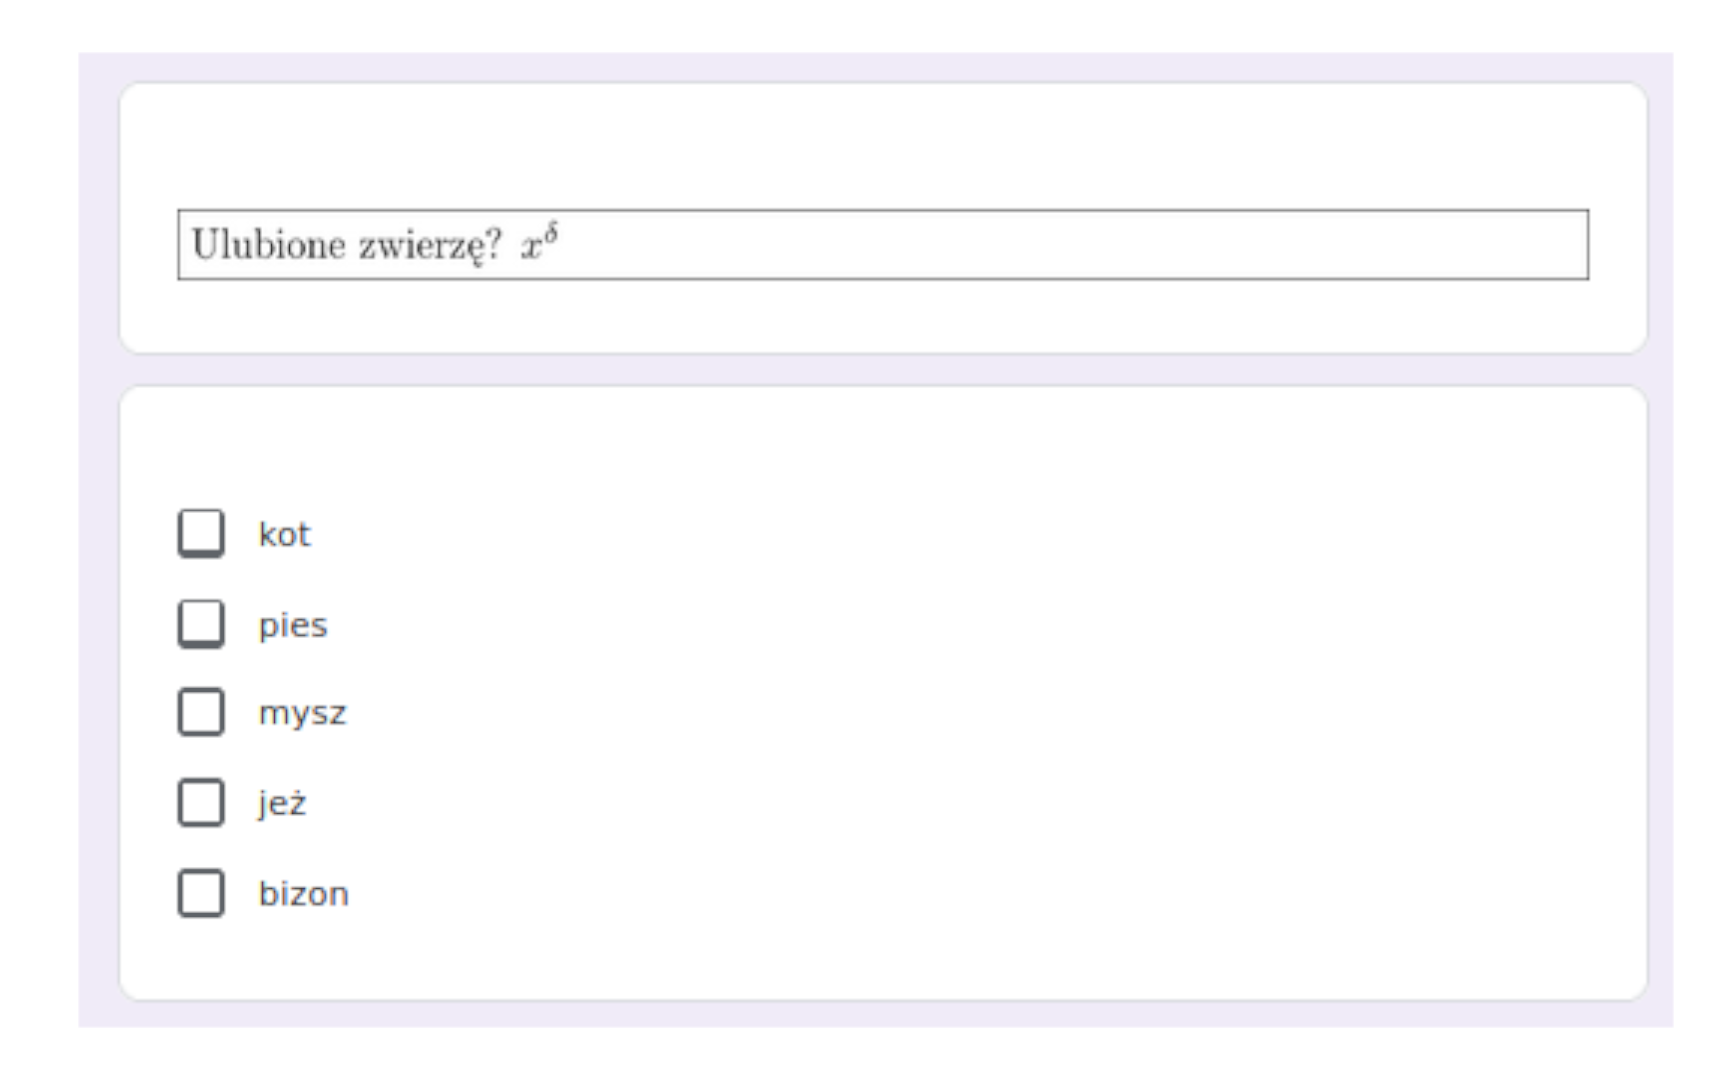
\includegraphics[scale=0.75]{przyklad.png}
  \caption{Przykład}
  \label{fig:1}
\end{figure}
Takie rozwiązanie wynika z ograniczeń  API formularzy, które nie udostępnia metod wprowadzenia zdjęć do popularnych typów pytań -- jest to znany problem, zgłaszany tutaj: \href{https://issuetracker.google.com/issues/36765518?pli=1}{https://issuetracker.google.com/issues/36765518?pli=1}. Metoda \textit{image} tworzy pole zdjęciowe w formularzu. 
Funkcja \textit{setFromFeatures} modyfikuje ustawienia formularza -- chodzi tu o zapamiętywanie adresów mailowych użytkowników przesyłających odpowiedzi, limit odpowiedzi na użytkownika, ustawienie współwłaściciela formularza oraz wartości, czy formularz powinien być oceniany automatycznie.
\ind Główną funkcją w pliku jest \textit{createFromJSON}, która generuje formularz poprzez wywoływanie odpowiednich metod z wymienionych wyżej. Właścicielem formularza jest właściciel aplikacji internetowej (użytkownik Google, pod którego  kontem tworzone są formularze). Takie rozwiązanie pozwala na uniknięcie potrzeby autoryzacji przy każdym dostępie do aplikacji internetowej.

\section{Konwersja wstawek z \LaTeX{}'a}
Niniejsza część korzysta z podstawowej biblioteki \LaTeX{}'a, szablon tworzonych zdjęć stanowi plik \textit{texTemplate.tex}. Wszystkie tworzone pliki znajdują się w folderze \textit{pictures}.
\ind Decyzja o napisaniu tej części w Pythonie powstała stosunkowo późno. Powodem jest biblioteka openCV -- udostępniająca zaawansowane metody obliczeniowe w przystępny sposób. Skrypt działa następująco:
\begin{itemize}
\item Wczytywany jest szablon w \LaTeX{}'u i w odpowiednie miejsce wstawiany jest tekst z pytania (oznaczonego tex=true) -- warto wspomnieć, że treść pytania jest otoczona ramką.
\item Za pomocą biblioteki tex2pix plik .tex jest konwertowany do formatu pdf.
\item Biblioteka pdf2image konwertuje pdf'a do png.
\item Biblioteka openCV pozwala na ,,wycięcie'' ze zdjęcia wyłącznie obszaru otoczonego ramką (jako jedyny zawiera kolory).
\item ,,Ramka'' jest zapisywana jako png.
\item Przy użyciu biblioteki base64 końcowe zdjęcie jest konwertowane do formatu base64 i zapisywane do pliku.
\item Pośrednie stadia konwersji są usuwane z folderu.
\end{itemize}
\subsection{Alternatywne rozwiązanie}%o tym czemu nie mathjax
Wydaje się naturalne, aby do problemu parsowania symboli matematycznych użyć gotowego silnika (opartego np. na Markdown'ie lub \LaTeX{}'u). Takim silnikiem jest na przykład MathJax. Udostępnia bogate API, integrację Webową. Doskonale współpracuje z JavaScriptem. Główną komplikacją jest to, że zwracany wynik jest w HTMLu -- co wymagałoby dodatkowej konwersji. Nie wykluczone jednak, że istnieje znacząco prostsze rozwiązanie - korzystające właśnie z takiego silnika.
\section{Skrypty instalujący i uruchamiający}
Instalacja oparta jest na npm (dla Node.js) i pip (Python) -- skrypt \textit{install.sh} instaluje wymagane biblioteki przy pomocy tychże narzędzi.
\ind  Uruchomienie programu wymaga uruchomienia dwóch części -- serwera lokalnego oraz interfejsu -- ten drugi wymaga przeglądarki internetowej. Skrypt \textit{run.sh} wypisuje ścieżkę pliku stanowiącego interfejs z prośbą o otwarcie go w przeglądarce i uruchamia serwer lokalny.










